% Required in preamble:
%   \usepackage{tikz}
%   \usetikzlibrary{arrows.meta,positioning,fit,backgrounds,calc}
\usetikzlibrary{arrows.meta,positioning,fit,backgrounds,calc}

% ── Node & arrow style definitions ──────────────────────────────────────────
\tikzset{
  %-- module: processing / algorithmic component (blue)
  module/.style={
    draw=blue!55!black, line width=0.65pt,
    rounded corners=3pt,
    fill=blue!18,
    minimum height=9mm,
    text width=2.75cm,
    align=center,
    font=\footnotesize
  },
  %-- data: data store / artifact (green)
  data/.style={
    draw=green!55!black, line width=0.65pt,
    rounded corners=3pt,
    fill=green!18,
    minimum height=9mm,
    text width=2.75cm,
    align=center,
    font=\footnotesize
  },
  %-- subsystem: grouping box (dashed gray)
  subsystem/.style={
    draw=gray!55, line width=0.7pt,
    dashed,
    rounded corners=5pt,
    fill=gray!7,
    inner sep=14pt
  },
  %-- Arrow: data pipeline (solid green)
  dataarrow/.style={
    -{Latex[length=2.4mm,width=1.7mm]},
    line width=0.8pt,
    draw=green!55!black
  },
  %-- Arrow: agent <-> env interaction (solid blue)
  agentarrow/.style={
    -{Latex[length=2.4mm,width=1.7mm]},
    line width=0.8pt,
    draw=blue!60!black
  },
  %-- Arrow: logging / artifacts (dashed gray)
  logarrow/.style={
    -{Latex[length=2.4mm,width=1.7mm]},
    line width=0.7pt,
    dashed,
    draw=gray!55
  },
  %-- Arrow: general control / data flow (black)
  flowarrow/.style={
    -{Latex[length=2.4mm,width=1.7mm]},
    line width=0.8pt,
    draw=black!65
  }
}

% ── Figure ───────────────────────────────────────────────────────────────────
\begin{figure*}[!tbp]
\centering
% node distance = <vertical gap> and <horizontal gap>
% All gaps are measured between node borders (positioning library semantics).
\begin{tikzpicture}[node distance=9mm and 11mm]

% ─────────────────────────────────────────────────────────────────────────────
% ROW 1  ·  Experiment Configuration
% Two nodes, left-aligned with the data pipeline below.
% ─────────────────────────────────────────────────────────────────────────────
\node[data] (configs)
  {\textbf{configs/*}\\base, agents, features, exps};

\node[module, right=of configs] (runner)
  {\textbf{Experiment Runner}\\run\_experiment.py};

% ─────────────────────────────────────────────────────────────────────────────
% ROW 2  ·  Data Pipeline
% Four nodes spanning full width.  Col alignment is guaranteed because each
% node's text width is identical, so right=of advances by the same delta.
% ─────────────────────────────────────────────────────────────────────────────
\node[data,   below=20mm of configs] (raw)
  {\textbf{Raw Market Data}\\EURUSD, GBPUSD, USDJPY, AUDUSD};

\node[module, right=of raw] (prep)
  {\textbf{Loader \& Preprocess}\\clean, align, adjust};

\node[module, right=of prep] (feat)
  {\textbf{Feature Engineering}\\technical + microstructure};

\node[data,   right=of feat] (dataset)
  {\textbf{Dataset Builder}\\train\,,/\,test splits};

% ─────────────────────────────────────────────────────────────────────────────
% ROWS 3–4  ·  Training System (cols 1–2) + Evaluation (col 4)
% Anchoring env below raw AND backtest below dataset guarantees shared
% vertical levels for rows 3 and 4 on both sides of the diagram.
% ─────────────────────────────────────────────────────────────────────────────

%-- Training row 3
\node[module, below=20mm of raw] (env)
  {\textbf{Trading Env}\\execution + reward};

\node[module, right=of env] (agent)
  {\textbf{RL Agent}\\DQN\,/\,Double DQN};

%-- Evaluation row 3 (col 4, same vertical level as env/agent)
\node[module, below=20mm of dataset] (backtest)
  {\textbf{Backtest Engine}\\deterministic rollout};

%-- Training row 4
\node[module, below=9mm of env] (replay)
  {\textbf{Replay Buffer}\\experience memory};

\node[module, right=of replay] (trainer)
  {\textbf{Trainer}\\updates + target sync};

%-- Evaluation row 4 (col 4, same vertical level as replay/trainer)
\node[module, below=9mm of backtest] (metrics)
  {\textbf{Metrics}\\return, Sharpe, MDD};

% ─────────────────────────────────────────────────────────────────────────────
% ROW 5  ·  Logging & Artifacts
% ─────────────────────────────────────────────────────────────────────────────
\node[module, below=20mm of replay] (artifact)
  {\textbf{Artifact Manager}\\checkpoints, configs};

\node[module, right=of artifact] (logging)
  {\textbf{Logging}\\train/eval + TensorBoard};

\node[module, right=of logging] (repro)
  {\textbf{Reproducibility}\\seeding, diagnostics};

% ─────────────────────────────────────────────────────────────────────────────
% ARROWS
% ─────────────────────────────────────────────────────────────────────────────

%-- Experiment config / control flow ----------------------------------------
\draw[flowarrow] (configs) -- (runner);
% runner sits at col 2; prep also at col 2 → perfectly straight vertical
\draw[flowarrow] (runner.south) -- (prep.north);

%-- Data pipeline (solid green) ---------------------------------------------
\draw[dataarrow] (raw)  -- node[above,font=\footnotesize]{load}  (prep);
\draw[dataarrow] (prep) -- node[above,font=\footnotesize]{feats} (feat);
\draw[dataarrow] (feat) -- node[above,font=\footnotesize]{split} (dataset);

%-- Dataset → Evaluation: direct vertical (offset +1.5 mm to fork cleanly)
\draw[flowarrow] ([xshift=1.5mm]dataset.south)
  -- node[right,font=\footnotesize]{eval} ([xshift=1.5mm]backtest.north);

%-- Dataset → Training Env: western-margin bypass
%   Path: dataset.south  ─(down 5 mm into R2–R3 gap)─
%         ─(horizontal left to left-margin waypoint)─
%         ─(vertical down to env's y)─
%         ─(short horizontal right into env.west)
\coordinate (westEntry) at ($(env.west)+(-9mm,0)$);
\draw[flowarrow]
  ([xshift=-1.5mm]dataset.south)
  -- ++(0,-5mm)
  -| (westEntry)
  -- node[above,font=\footnotesize]{train} (env.west);

%-- Environment ↔ Agent: dual offset lanes (solid blue) --------------------
\draw[agentarrow]
  ([yshift= 2mm]env.east)
  -- node[above,font=\footnotesize,text=blue!65!black]{obs}
  ([yshift= 2mm]agent.west);

\draw[agentarrow]
  ([yshift=-2mm]agent.west)
  -- node[below,font=\footnotesize,text=blue!65!black]{action}
  ([yshift=-2mm]env.east);

%-- Training internals
\draw[flowarrow] (env.south)   -- (replay.north);
\draw[flowarrow] (replay.east) -- node[above,font=\footnotesize]{transitions} (trainer.west);
\draw[flowarrow] (agent.south) -- node[right,font=\footnotesize]{policy} (trainer.north);

%-- Evaluation chain
\draw[flowarrow] (backtest.south) -- node[right,font=\footnotesize]{stats} (metrics.north);

%-- Logging flows (dashed gray)
%   trainer → logging: offset +1.5 mm east, straight vertical
\draw[logarrow]
  ([xshift= 1.5mm]trainer.south)
  -- ++(0,-3mm)
  -| node[below right,font=\footnotesize]{log}
  (logging.north);

%   trainer → artifact: route through R4–R5 gap, then left to artifact
\draw[logarrow]
  ([xshift=-1.5mm]trainer.south)
  -- ++(0,-5mm)
  -| node[above,font=\footnotesize]{ckpt}
  (artifact.north);

%   metrics → logging: route through R4–R5 gap (staggered at −4.5 mm
%   to avoid the trainer→logging horizontal at −3 mm)
\draw[logarrow]
  (metrics.south)
  -- ++(0,-4.5mm)
  -| node[above,font=\footnotesize]{eval}
  (logging.east);

% ─────────────────────────────────────────────────────────────────────────────
% BACKGROUND SUBSYSTEM BOXES
% fit= auto-sizes each box; labels anchor inside the box border.
% ─────────────────────────────────────────────────────────────────────────────
\begin{scope}[on background layer]

  \node[subsystem,
    fit=(configs)(runner),
    label={[anchor=north west,font=\bfseries\footnotesize,text=black!70]
      north west:\strut 1.~Experiment Configuration}] {};

  \node[subsystem,
    fit=(raw)(prep)(feat)(dataset),
    label={[anchor=north west,font=\bfseries\footnotesize,text=black!70]
      north west:\strut 2.~Data Pipeline}] {};

  \node[subsystem,
    fit=(env)(agent)(replay)(trainer),
    label={[anchor=north west,font=\bfseries\footnotesize,text=black!70]
      north west:\strut 3.~Training System}] {};

  \node[subsystem,
    fit=(backtest)(metrics),
    label={[anchor=north west,font=\bfseries\footnotesize,text=black!70]
      north west:\strut 4.~Evaluation}] {};

  \node[subsystem,
    fit=(artifact)(logging)(repro),
    label={[anchor=north west,font=\bfseries\footnotesize,text=black!70]
      north west:\strut 5.~Logging \& Artifacts}] {};

\end{scope}

% ─────────────────────────────────────────────────────────────────────────────
% LEGEND
% Centered below Row 5, using the midpoint between leftmost and rightmost
% bottom nodes so the legend self-adjusts if nodes are added/removed.
% ─────────────────────────────────────────────────────────────────────────────
\node[
  draw=gray!50, rounded corners=3pt, fill=white,
  inner sep=7pt,
  font=\footnotesize,
  anchor=north,
] (legend) at ($(artifact.south)!0.5!(metrics.south)+(0,-24mm)$)
{%
  \renewcommand{\arraystretch}{1.18}%
  \begin{tabular}{@{}c@{\hspace{6pt}}l@{\hspace{14pt}}c@{\hspace{6pt}}l@{}}
    % ── Arrow types ──────────────────────────────────────────────────
    \begin{tikzpicture}[baseline=-0.5ex]
      \draw[dataarrow]  (0,0)--(10mm,0);
    \end{tikzpicture}
    & Data pipeline
    &
    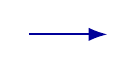
\begin{tikzpicture}[baseline=-0.5ex]
      \draw[agentarrow] (0,0)--(10mm,0);
    \end{tikzpicture}
    & Agent\,$\leftrightarrow$\,Env
    \\
    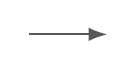
\begin{tikzpicture}[baseline=-0.5ex]
      \draw[flowarrow]  (0,0)--(10mm,0);
    \end{tikzpicture}
    & Control flow
    &
    
\begin{tikzpicture}[baseline=-0.5ex]
      \draw[logarrow]   (0,0)--(10mm,0);
    \end{tikzpicture}
    & Logging / artifact
    \\
    % ── Node types ───────────────────────────────────────────────────
    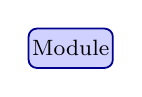
\begin{tikzpicture}[baseline=-0.5ex]
      \node[module, minimum height=5mm, text width=10mm,
          font=\footnotesize, inner sep=1pt]{Module};
    \end{tikzpicture}
    & Module (blue)
    &
    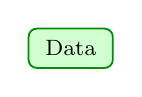
\begin{tikzpicture}[baseline=-0.5ex]
      \node[data, minimum height=5mm, text width=10mm,
          font=\footnotesize, inner sep=1pt]{Data};
    \end{tikzpicture}
    & Data node (green)
    \\
  \end{tabular}%
};

\end{tikzpicture}

\caption{System architecture of the RL trading framework, linking configuration, data processing, training, deterministic backtesting, and reproducibility logging in one end-to-end pipeline.}
\label{fig:system_architecture}

\end{figure*}